\chapter{Heqsim: Heterogeneous Quantum Computing Simulator}

\section{About}

Heqsim is a distributed quantum computing simulator that the author is developing, and will be an open-source Python library after some minor bugs will be fixed (The GitHub repository is private right now).  Currently, this simulator has the following features such as 

\begin{itemize}
      \item Users can specify different execution time per gate to each quantum processor
      \item Users can also specify the network topology among quantum processors 
\end{itemize}
.
Heqsim is the first distributed quantum computing simulator that have these features.  The existing distributed quantum computing simulator NetQuil \cite{netquil} and Inter-linq \cite{parekh} , both of which are only restricted to fully-connected network topology.

\newpage

\section{How Heqsim works}

Here is the procedure of the simulation using heqsim.

\begin{figure}[h]
  		\begin{center}
  			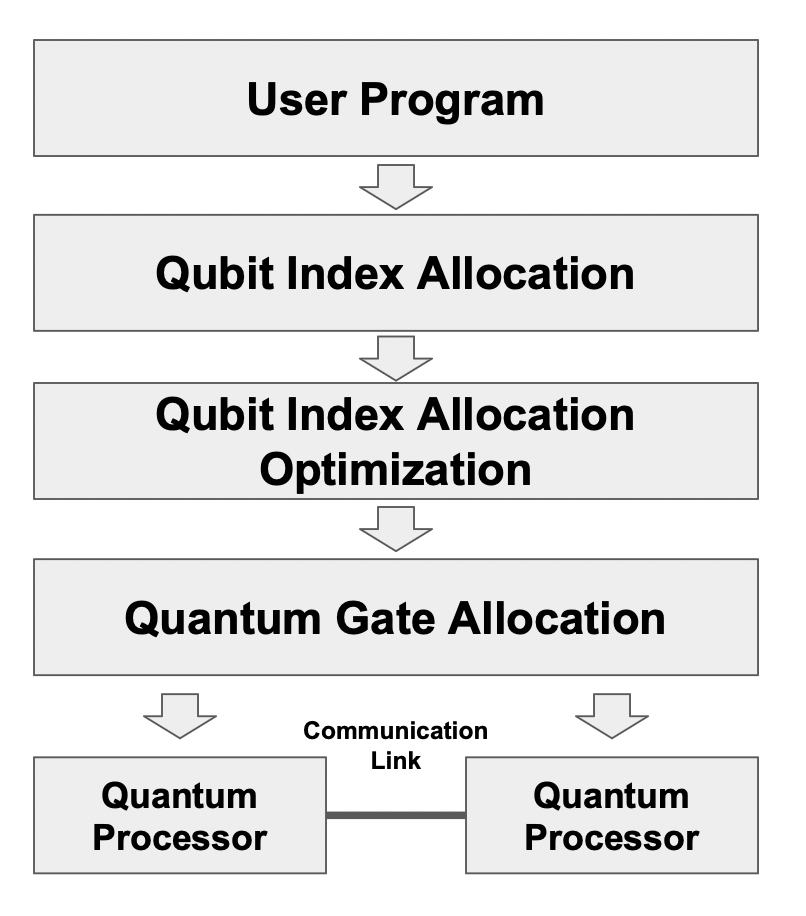
\includegraphics[width=8cm]{img/procedure.png}
			\caption{Procedure of heqsim simulation}
		\end{center}
\end{figure}.

\subsection{User Program}

Users can specify the details (number of qubits, execution time) of each quantum processor and the network topology of the entire quantum computing cluster.  Also, they can specify the quantum circuit that they want to implement.

\subsection{Qubit Index Allocation}

Heqsim receives the information of the total qubits in the given quantum circuit and distributes each qubit to random quantum processors. 

\subsection{Qubit Index Allocation Optimization}

The Qubit Allocation Optimizer optimized the qubit index allocation by using the method described in the previous chapter.

\subsection{Quantum Gate Allocation Optimization}

The module called Gate Allocator distributed quantum gates according to the result of qubit index allocator and also decomposes some CNOT gates according to the network topology.

\subsection{Quantum Processor}

Quantum Processor applies actual quantum gates given by the gate allocator.  The single gates are implemented by parallel execution, but communication is emulated by communication links between two quantum processors.
